\documentclass[11pt]{report}
\usepackage{fullpage}
\usepackage{graphicx}
%\usepackage{longtable}
%\usepackage{multirow}
\usepackage{psfig}
\usepackage{amsmath}
%\usepackage{amsthm}
%\usepackage{amsfonts}
%\usepackage{amssymb}
\usepackage{times} 
\usepackage{url}

\newcommand{\comment}[1]{\textit{\small {#1}}}
\newcommand{\cpp}{C\texttt{++}\ }
\newcommand{\tcl}{\textsc{Tcl\ }}
\newcommand{\ProtoMol}{\textsc{ProtoMol }}
\newcommand{\MDL}{\textsc{MDL\ }}
\newcommand{\MOLLY}{\textsc{MOLLY\ }}

\newcommand{\tempstart}{\texttt{<}}
\newcommand{\tempend}{\texttt{>}}
\newcommand{\rij}{\mbox{r$_{ij}$}}
\newcommand{\rik}{\mbox{r$_{ik}$}}
\newcommand{\vrij}{\mbox{$\vec{r}_{ij}$}}
\newcommand{\Si}[1]{\mbox{Si$_{#1}$}}
\newcommand{\Vr}[1]{\mbox{$\vec{r}_{#1}$}}
\newcommand{\Vx}[1]{\mbox{$\vec{x}_{#1}$}}
\newcommand{\Vv}[1]{\mbox{$\vec{v}_{#1}$}}
\newcommand{\hatr}[1]{\mbox{$\hat{{r}_{#1}}$}}
\newcommand{\hatv}[1]{\mbox{$\hat{{v}_{#1}}$}}
\newcommand{\AbsVr}[1]{\mbox{$\left| \vec{r}_{#1} \right| $}}
\newcommand{\AbsVv}[1]{\mbox{$\left| \vec{v}_{#1} \right| $}}
\providecommand{\textinmath}[1]{\mbox{#1}}
\providecommand{\ttsmall}[1]{\texttt{\small\mbox{#1}}}

\renewcommand{\labelenumiii}{\arabic{enumiii}.}
%%%%%%%%%%%%%%%%%%%%%%%%%%%%%%%%%%%%%%%%%%%%%%%%%%%%%%%%%%%%%%%%%%%%%%%%%

\author{
%  \begin{tabular}{cc}
%   Jes\'{u}s A. Izaguirre       & Thierry Matthey \\
%   Department of Computer Science      & Department of Informatics\\
%   University of Notre Dame      & University of Bergen \\
%     USA               & Norway \\
%    {\it izaguirr@cse.nd.edu} & {\it matthey@ii.uib.no} \\
%        &
%  \end{tabular}\\ \\ \\
%  \centerline{\ttsmall{http://www.nd.edu/\~{ }lcls}}\\
%  \centerline{\it protomol@cse.nd.edu}\\ 
%  ~\\ \\
  \centerline{Authors: Trevor Cickovski, Chris Sweet and Jes\'{u}s A. Izaguirre}\\ \\ \\
%  \centerline{Atul Bahel}\\ \\ \\
%  \centerline{Trevor Cickovski}\\
%  \centerline{Scott Hampton}\\
%  \centerline{Hong Hu}\\
%  \centerline{Qun Ma}\\
%  \centerline{Branden Moore}\\
%  \centerline{Thomas Slabach}\\
%  \centerline{Jeffrey Stine}\\
%  \centerline{George Viamontes}\\
%  \centerline{Jeremiah Willcock}\\
%~\\ \\ \\
%  \centerline{Edited by:} \\ \\
%  \centerline{Jim Bilek} \\ \\
}
\title{\MDL - User Guide}

%%%%%%%%%%%%%%%%%%%%%%%%%%%%%%%%%%%%%%%%%%%%%%%%%%%%%%%%%%%%%%%%%%%%%%%%%
\begin{document}
\maketitle
\tableofcontents

%%%%%%%%%%%%%%%%%%%%%%%%%%%%%%%%%%%%%%%%%%%%%%%%%%%%%%%%%%%%%%%%%%%%%%%%%

\begin{abstract}

Molecular Dynamics (MD) involves solving Newton's equations of motion
for a system of atoms, using the resulting forces to propagate the
system in time.  Since the most computationally intensive calculations
of MD simulations (i.e., pairwise force evaluations) yield great
difficulty in modeling systems of reasonable size for a biologically
relevant period of time, an important area of research
is the development of efficient numerical methods for MD simulations.  
The Molecular Dynamics Lab (MDL) is designed for the prototyping, testing 
and debugging of these methods, built with the scripting 
language Python.

The user guide begins with a description of the features of MDL,
followed by a guide to constructing MD simulations protocols for
the purposes of testing numerical methods and interacting with external
tools for data analysis.  Following is a description of how to construct
new propagators and force calculators.  It concludes with some helpful
examples, other necesssary background on MD, and software
licensing.

\end{abstract}


\chapter{Introduction}

MD simulations can be instrumental to understanding the short and
long-term behavior of molecular systems, which holds implications 
for fields such as drug design, protein folding and the human
genome project.  Although researchers currently possess 
high-performance and optimized software running on parallel 
supercomputing clusters, it is extremely difficult to model systems
of reasonable size for a biological time which exceeds the microsecond
timescale, well short of desirable for protein folding which
occurs on the second timescale.  This is due mainly to two factors:
(1) high-frequency motions (i.e., bond fluctuations) within a molecule
which limit the propagation timestep, and (2) the quadratic algorithm
for pairwise force computation.

Given these limitations which still exist with high performance
computing, the continued development of efficient numerical
methods for MD simulations is very important.  We have seen
for instance restraints such as SHAKE \cite{GUNS77} and RATTLE \cite{Ande83}
which afford larger timesteps by restraining fast frequency
motions.  Multiple timestepping propagators calculate different
forces at different frequencies depending on how fast they
vary.  In Normal Mode Analysis \cite{}, motions are split into
fast and slow frequencies, with fast frequencies oscillating
around 'normal' values.  Fast electrostatic methods such as Ewald \cite{Ewal21}
and PME \cite{DaYP93} improve the quadratic complexity of evaluating
coulombic interactions at a cost of some accuracy.


It thus makes sense to provide a tool which can above all facilitate 
construction of these methods, and the ability to test and debug with 
realistic biological systems and conduct parameter sweeps.  But this can
be difficult using a framework designed for performance because these
tend to be written in languages such as FORTRAN or C which do
not cater well to extensibility.  Scripting languages make it easier
to construct programs quicker and on the fly and are often interpreted,
which avoids the need to reproduce machine code upon modifications.
Python contains several features which cater well to testing and debugging
such as dynamic typing and dynamic binding, and is also portable
and readable.  Moreoever there is an abundance of external tools built
 with Python which become interfacable to MDLab as a result.


This User Guide provides a summary for the operation of MDLab,
including construction of simulation protocols, propagators and
force calculators.  MDL currently possesses the following capabilities:

\begin{enumerate}
\item {\bf Compatibility with CHARMM force fields}.  Construction
of a physical system in MDL involves reading CHARMM \cite{Broo83} Protein
Structure Files (PSFs) and Parameter (PAR) files.  Files from the 
Protein Data Bank (PDB, \cite{BERN77}) can be used to populate atomic positions.
Pairwise computations such as the Lennard-Jones potential \cite{} which
models both van der Waals and Pauli Exclusion force terms, and the
electrostatic forces are customizable through evaluation algorithms, cutoffs
and switching functions.
\item {\bf Construct a physical system}. MDL provides the ability
for a user to control parameters such as simulation boundary conditions, 
Kelvin temperature, etc. along with easy access to observables such
as the atomic position and velocity vectors, mass matrices, and cell
basis vectors which are constructed as Numpy \cite{NUMP05} arrays for
optimized matrix-vector operations.
\item {\bf Construct propagators and force calculators}. MDL provides
several known MD propagators and evaluation of terms from CHARMM
force fields.  These exist as precompiled shared object binaries
for maximum performance.  Alternatively, propagators and force calculators
can be built using constructs provided by Python modules within the MDL
package along with mathematical operations on simulation data.  
MDL makes use of {\it factories} \cite{Alex01} which uniquely
map Python strings to propagators and force calculators, enabling easy
access from simulation protocols.
\item {\bf Perform data analysis}. MDL provides several opportunities
for data analysis.  This can be done through file output, which includes
binary DCD trajectory files, screen output, or Matlab \cite{MATH05}-compatible
data charts.  Through Gnuplot-py \cite{GNUP05} or Matplotlib \cite{MATP05}, MDL can
plot observables such as temperature, pressure, total energy or potential
terms, etc. which makes verification of propagation schemes easier; for
example by ensuring conserved quantity fluctuations remain bounded.
Finally, MDL can interact with the Java GUI of ProtoMol (see \cite{Matt04}),
which can interactively visualize a system while running MDL commands
in the background.  MDL is actually part of a larger Problem Solving
Environment (PSE, \cite{GaHR94, MHK+06}) ProtoMol which also contains a computational back
end, for which MDL serves as a {\it scripting interface}.  This is convenient
since expansions to the computational back end become available in MDL.
\end{enumerate}


\chapter{Setting Things Up}

MDL is distributed as a part of the ProtoMol framework, which is available
open source on SourceForge (\texttt{http://www.sourceforge.net}).  The latest
version of the source code for MDL and the ProtoMol back end are available
using Subversion \cite{SUBV07}, and can be checked out by running the
following:

\begin{verbatim}
svn co https://protomol.svn.sourceforge.net/svnroot/protomol protomol
\end{verbatim}

This will provide you with anonymous read access to the svn repository,
from which you can obtain source code updates using \texttt{svn update}.
The MDL framework is contained within the directory \texttt{protomol/mdl},
but is coupled to the ProtoMol computational back end in that the
functionality of several C++ files has been wrapped for Python using
SWIG \cite{Beaz96}, which also generates C function implementations
as precompiled shared object libraries.  To use MDL, you will need 
to install some external tools, which we outline below as prerequisites.
Although there seems to be quite a few prerequisites, you may have some
of them already and they are all relatively easy to install and do
not themselves require other dependencies.  So you should be able
to have everythin set up in a relatively short period of time.

\section{Prerequisites}

Here we provide a set of tools which are required to execute MDL.
Some of them may be installed on your machine already.  However,
they may not be the correct versions, and you should check to make
sure that the version of each tool corresponds to the version
specified below.  Please install these tools in the order they
appear.

\subsection{Python 2.5}

The Python interpreter should come standard on most versions of *nix
and some versions of Mac OS.  If Python has been installed, you can
check the version by starting the Python interpeter and passing
the \texttt{-V} flag, like so:

\begin{verbatim}
python -V
\end{verbatim}

The version printed should be minimally Python 2.5.  If it is not,
you will need to install an updated version.  Python is available
open source at \texttt{http://www.python.org}.  Follow instructions
under 'Download'.  The safest bet is to download Python 2.5 since
this is the version used by developers; although future versions
should be back-compatible.

\subsection{SCons}

SCons (\texttt{http://www.scons.org}) is a software construction
tool built entirely in Python which offers an alternative to Makefiles
for compiling source code and linking software applications.  Follow
the instructions for downloading version 0.98.  
You will use this to compile the ProtoMol back end into a shared 
object binary which will dynamically link to the shared libraries 
imported by MDL.

\subsection{SWIG}

SWIG (Simplified Wrapper Interface Generator, \cite{Beaz96} is an
open source tool which can generate wrapper code for C and C++
entities in many different languages (many of them scripting
languages), Python being one of them.  SWIG does come standard
on many versions of *nix, but to use MDL you will minimially
need version 1.3.31.  You can check your version number by
executing:

\begin{verbatim}
swig -version
\end{verbatim}

If you do not have at least 1.3.31, you can download SWIG
from \texttt{www.swig.org}.  Follow the instructions, and make
sure you check C++ as your input language and Python as you target,
and select your appropriate platform.

\subsection{Numpy}

Numerical Python (NumPy, \texttt{http://numpy.scipy.org/}) is
available open source and provides a set of libraries implemented
in Python for scientific computing.  Most importantly, NumPy
matrix-vector operations are powerful and optimized, which
are critical for MD simulations.  Follow the directions for
basic installation; there is no need to include any prefixes as
the built NumPy libraries will be deposited in your Python
installation.

\subsection{Gnuplot-py or Matplotlib}

Gnuplot-py is a plotting library built in Python which
interfaces to the Gnuplot utility and can plot data
interactively.  On *nix, to make sure you have Gnuplot
installed execute \texttt{which gnuplot} and make sure
there is an application installed.  Then follow the 
instructions from \texttt{http://gnuplot-py.sourceforge.net/}
to complete the installation.  Once again, install in the default
location so that the installation will deposited in your
Python installation.

Alternatively to Gnuplot-py, you can choose to install
Matplotlib if you are certain that will most often be your
plotting tool.  Since however plotting with Matplotlib
is not the default, we recommend also installing Gnuplot-py
since it's fast and easy, but if you choose to only install
Matplotlib you will need to indicate this in your simulation
protocols.  Matplotlib is available open source at
\texttt{http://matplotlib.sourceforge.net}.

\section{Installation}

Once you have these tools, you are ready to install and
run MDL.  The first step will be to change to the ProtoMol
root directory, and type:

\begin{verbatim}
scons mdl=1 lapack=1 gui=1
\end{verbatim}

The three flags here indicate: (1) that you intend to compile
ProtoMol as a shared object file to be dynamically loaded for 
MDL and that you want appropriate ProtoMol classes and functions
SWIG-wrapped for Python, (2) that you want to link in Lapack \cite{}
functionality, and (3) that you would like to potentially
use the Java GUI for interactive visualization of MDL simulations.
The \texttt{lapack} flag only comes into play for normal
mode propagators, so if you do not see yourself using those you
can leave this flag out.  We recommend however including everything
possible at the point of compilation, since if you later change
your mind you will have to recreate the shared object file which
can take some time.

Once the compilation is finished, you are ready to use MDL.
The three basic types of Python scripts that MDL is built to handle
are simulation protocols, propagator classes and functions, and
force classes.  We recommend reading the next section on simulation
protocols and actually running MDL per the instructions in the
next section, to get accustomed to the organization and procedures
of the MDL framework.

\chapter{Simulation Protocols}

The basic facility for testing numerical methods will be an MDL
{\it simulation protocol}, which involves setting up a biological
system and propagating it with time.  Protocols can be run through
a standard Python interpreter.  However, prior to execution it is 
necessary for the interpreter to know the location of MDL modules
for importing, contained within the environment variable 
\texttt{PYTHONPATH}.  MDL provides two files for properly
setting up your \texttt{PYTHONPATH}: \\

1. MDLSetup.bash (for bash users) \\
\indent 2. MDLSetup.tcsh (for csh or tcsh users) \\

If you are unsure of your shell, type in a terminal:

\texttt{printenv SHELL}\\

MDL contains several example simulation protocols within
the \texttt{simulations/} folder, as Python scripts runnable
through:

\texttt{python simulations/<file>.py}\\

You may also set up your own simulation protocol but the structure
will be similar to the examples provided.  We will now run through
the 'typical' structure of an MDL simulation protocol.

\section{Importing Core Modules}

A Python module is implemented within its own Python script
and contained classes and functions applicable to a specific
task.  MDL provides five 'core' Python modules which are each
responsible for a separate portion of an MD simulation:

\begin{enumerate}
\item {\bf Physical}: The physical system, consisting of atomic positions
and velocities, mass and inverse mass matrices, boundary conditions
and cell basis vectors (if applicable), Kelvin temperature, and
biological time.
\item {\bf IO}: Provides functionality for reading and writing data.
This includes readers for file input when constructing the physical
system, and output for data analysis including plots, screen, and 
files.
\item {\bf Forces}: Contains the atomic force vector and each type
of energy: kinetic and potential, including individual components 
(two-atom bond fluctuation potential, three atom angle, etc.).
\item {\bf ForceField}: Contains a group of forces to evaluate.  These forces
can be CHARMM forces (bond, angle, dihedral, improper, Lennard-Jones
and electrostatic), or Python-prototyped force calculators.
\item {\bf Propagator}: Provides methods for propagating a system with time.
\end{enumerate}

An MD simulation protocol will most likely need everything
from these five modules, so the first step will typically be to
import all of their functionality using the Python interpreter:

\begin{verbatim}
from Physical import *
from Forces import *
from ForceField import *
from IO import *
from Propagator import *
\end{verbatim}

\section{Physical System}

An MD simulation will always consist of some sort of biological
system, that is being propagated with time.  MDL provides several
example systems in the \texttt{data/} directory.  These include: \\

%\begin{enumerate}
\noindent 1. Alanine dipeptide in vacuum (22 atoms).\\
2. Solvated alanine (22 atom solute, 445 water molecules).\\
3. Block alanine dipeptide in vacuum (22 atom block structure).\\
4. Two argon systems (ideal gas, 280 and 400 molecules).\\
5. Two solvated bovine pancreatic tripsin inhibitor (882 and 898 atom solute, 73 and 4461 water molecules).\\
6. Decalanine in vacuum (66 atoms).\\
7. United atom butane in vacuum (4 atoms).\\
8. Two water boxes (72 and 216 water molecules).\\
9. The WW domain (551 atoms).\\
%\end{enumerate}

\subsection{Requirements}

The physical system describes attributes of the 
molecular system such as structure, coordinates, 
boundary conditions, pairwise exclusions, and temperature.
Many of these attributes are defined within input files provided
in these example folders, in addition you can download new
example systems from the Protein Data Bank.  To define a physical
system in MDL, you will first want to declare a Python object
to contain this information.  In this case we use the variable
name \texttt{phys}, but you can use any valid Python variable
name to reference this object:

\begin{verbatim}
phys = Physical()
\end{verbatim}

For initial coordinates, structure, and force field parameters
you will want to use input files to populate the object.  To
access functionality for file I/O, you also must define an
\texttt{IO} object:

\begin{verbatim}
io = IO()
\end{verbatim}

Coordinates for positions and velocities can then be specified
using PDB files (from the Protein Data Bank) or XYZ files
(a simple format consisting of four columns - atom name, and
\begin{math} (x,y,z) \end{math} coordinates:

\begin{verbatim}
io.readPDBPos(phys, "examples/bpti_water_1101/bpti.pdb")
io.readXYZVel(phys, "examples/bpti_water_1101/bpti.vel.xyz")
\end{verbatim}

Initializing atomic positions is a requirement.  By invoking
\texttt{readPDBPos} or \texttt{readPDBVel}, the \texttt{positions}
data member of the passed \texttt{Physical} object will be populated.
The \texttt{positions} data member is a NumPy array of floating
point values, so it also can be populated manually if so desired.
Explicitly initializing atomic velocities is not a requirement, 
if an initial Kelvin temperature is provided then velocities
will be initialized using a Maxwell distribution with mean zero
and standard deviation equal to \begin{math}\frac{k_B T}{m}\end{math}.
This can be specified by referencing the \texttt{temperature}
attribute of \texttt{Physical}.  In addition, the \texttt{seed}
data member can be set to ensure random number consistency across 
simulations (it is by default 1234):

\begin{verbatim}
phys.temperature = 300 
phys.seed = 1769
\end{verbatim}

CHARMM parameter and PSF files specify structure and
extra information such as spring constants, equilibrium
lengths for bonds, etc.  These are required and can only be
populated through files:

\begin{verbatim}
io.readPSF(phys, "examples/bpti_water_1101/bpti.psf")
io.readPAR(phys, "examples/bpti_water_1101/bpti.par")
\end{verbatim}

This is the minimum necessary to set up an MDL physical
system, since default values are provided for other parameters.
However, you can manually specify these as well by directly
referencing member attributes of the \texttt{Physical} object.

\subsection{Other Attributes}

\begin{enumerate}

\item {\bf Boundary Conditions}.  
The \texttt{bc} data member of \texttt{Physical} is a Python
string which can either be set to \texttt{Periodic} (default)
or \texttt{Vacuum}.  Periodic boundary conditions implement
a wraparound at the edges of the simulation box, so that when
atomic pairwise distances are calculated the closer of either
straight-up Euclidean or wraparound will be used.  This is
useful for modeling the effects of an encompassing bulk solvent.
Vacuum simply computes Euclidean distance with no wraparound:

\begin{verbatim}
phys.bc = "Periodic"        # Boundary conditions
\end{verbatim}

\item {\bf Pairwise Exclusions}.  
Certain nonbonded pairwise force calculations can be excluded if
the same pairwise calculation is performed for a bonded potential.
The \texttt{exclude} attribute specifies the level of exclusion,
which is a Python string that can set to one of the following:
\texttt{1-2} (exclude all directly covalently bonded atom pairs),
\texttt{1-3} (1-2 plus exclude all atom pairs which share a covalently
bonded atom), \texttt{1-4} (1-3 plus exclude all atom pairs within
two covalent bonds of each other), \texttt{scaled1-4} (default, 1-4 but instead
of completely excluding atom pairs within two covalent bonds, scale
the nonbonded term down):

\begin{verbatim}
phys.exclude = "scaled1-4"  # Pairwise exclusion
\end{verbatim}

\item {\bf Cell Size}.
Internally, when computing pairwise forces MDL uses a routine
from ProtoMol which divides simulation space into {\it cells},
and a {\it cell manager} keeps track of the atoms within each
cell.  Since it is inefficient to recompute all pairwise distances
at every simulation step, only pairs of atoms within neighboring
cells are considered.  This will only make sense if a {\it cutoff}
is used for pairwise calculations (explained later), and then 
maximum efficiency can be obtained by setting the \texttt{Physical} 
attribute to twice the cutoff:

\begin{verbatim}
phys.cellsize = 4           # Periodic cell size
\end{verbatim}

\item {\bf Cell Basis Vectors}.
When using periodic boundary conditions, the dimensions of 
the periodic box are by default obtained by using the minimum
and maximum \begin{math}(x, y, z)\end{math} coordinates of 
the initial configuration, but this can be specified manually
by providing a set of three cell basis vectors which span the periodic
box, plus an origin.  These are contained within the \texttt{Physical}
attributes \texttt{cB1}, \texttt{cB2}, \texttt{cB3}, and \texttt{cO}
which are three-element numpy arrays of floating point values:

\begin{verbatim}
phys.cB1[0] = 29
phys.cB1[1] = 0
... etc ...
\end{verbatim}

\item {\bf Linear and Angular Momentum}.
The effects of collective system linear and angular momentum
can be removed at a given frequency using the \texttt{remcom}
(actually references the center of mass motion)
and \texttt{remang} attributes of \texttt{Physical}.  These can
hold values of -1 (never), 0 (once at the beginning), or 
an integer frequency in simulation steps.  Biologically, for
a single-timestepping propagation this time will be equal to
the frequency times the timestep \begin{math} \Delta t \end{math}:

\begin{verbatim}
phys.remcom = 2
phys.remang = 2
\end{verbatim}

\end{enumerate}

\section{Forces and Force Fields}

During any MDL simulation the atomic force vector
and energy values are obtainable through an MDL
\texttt{Forces} object, which can be constructed
similarly:

\begin{verbatim}
forces = Forces()
\end{verbatim}

Computed atomic forces are stored within the attribute
\texttt{force}, which is a numpy array of floating point values.
In addition, energies are stored within the attribute
\texttt{energies}, which provides the following methods
for accessing energy values: \\

%\begin{enumerate}
\noindent {\bf bondEnergy()}: Bond fluctuation potential.\\
{\bf angleEnergy()}: Potential resulting from deviations
of three-atom angles from equilibrium values.\\
{\bf dihedralEnergy()}: Potential resulting from deviations
of four-atom dihedrals from equilibrium values.\\
{\bf improperEnergy()}: Potential resulting from deviations
of four-atom impropers from equilibrium values.\\
{\bf ljEnergy()}: Lennard-Jones potential.\\
{\bf coulombEnergy()}: Electrostatic potential.\\
{\bf shadowEnergy()}: Shadow potential, if calculated.\\
{\bf potentialEnergy()}: Total potential energy, which is the sum
of the above terms.\\
{\bf kineticEnergy()}: Total kinetic energy.\\
{\bf totalEnergy()}: Total energy (potential+kinetic).\\
%\end{enumerate}


The \texttt{energies} data member also provides methods to
accumulate an energy quantity into one of the above terms,
with {\bf addBondEnergy(int)}, {\bf addAngleEnergy(int)}, etc.
These methods are useful when constructing Python forces, to
designate which energy term is effected by the resulting potential.

The \texttt{Forces} object contains calculated force and
energy data, and a \texttt{ForceField} object contains a specification
of which forces to evaluate.  A \texttt{ForceField} can
be constructed to evaluate CHARMM forces, which include
the following: \\

%\begin{enumerate}
* Two-atom bond forces, resulting from deviations from
equilibrium lengths.\\
\indent * Three-atom angle forces.\\
\indent * Four-atom dihedral and improper forces.\\
\indent * Van der Waals forces (using LennardJones evaluation).\\
\indent * Electrostatic or Coulombic forces.\\
%\end{enumerate}

If a \texttt{Forces} object has been defined, a \texttt{ForceField}
can be constructed by invoking its member function \texttt{makeForceField()},
passing a \texttt{Physical} object and the Python string \texttt{charmm}
to evaluate CHARMM forces.  To evaluate a subset (i.e. noble gas simulations
will not have bonded forces) or a different set of
forces, simply ignore the second argument:

\begin{verbatim}
forces = Forces()                           # Declare a Forces object
ff = forces.makeForceField(phys, "charmm")  # Return a ForceField
\end{verbatim}

You can evaluate a subset of CHARMM forces by using \texttt{ForceField}
member functions \texttt{bondedForces} and \texttt{nonbondedForces},
passing Python strings with uniquely identifying characters.
For bonded forces, ``b''=bond, ``a''=angle, ``d''=dihedral
and ``i''=improper.  For nonbonded, ``l''=van der Waals
and ``c''= electrostatic:

\begin{verbatim}
forces = Forces()                           # Declare a Forces object
ff = forces.makeForceField(phys)            # Return a ForceField
ff.bondedForces("bd")                       # Bond and dihedral
ff.nonbondedForces("l")                     # Van der Waals
\end{verbatim}

By default, all specified pairwise forces are evaluated
using a quadratic {\it direct} algorithm, meaning all pairs are
considered.  For CHARMM pairwise forces, MDL provides the opportunity to
change the {\it algorithm} for force evaluation, to \texttt{Cutoff}
for example.  In the case of \texttt{Cutoff}, after a certain
pairwise distance zero is assumed for the resulting potential, 
eliminating the need to evaluate pairwise force between atoms beyond
the distance and saving performance.  Parameters such as the algorithm
and cutoff value are accessible through the \texttt{params} data
member of \texttt{ForceField}, which is a Python dictionary:

\begin{verbatim}
# Cutoff the Lennard-Jones potential after 6.5 angstroms
ff.params = {'LennardJones':{'algorithm':'Cutoff',
                             'cutoff':6.5}}
\end{verbatim}

If both CHARMM Lennard-Jones and Coulomb forces are being evaluated,
and the same parameters are used for both, you can save performance
by setting both sets of parameters at the same time. In this case,
atomic pairs will be evaluated once for both, resulting in considerable
performance savings.  This is also the default:

\begin{verbatim}
# Cutoff the Lennard-Jones and electrostatic potential after 6.5 angstroms
ff.params = {'LennardJonesCoulomb':{'algorithm':'Cutoff',
                                    'cutoff':6.5}}
\end{verbatim}

An abrupt dropoff in the potential at the cutoff values can
cause numerical instabilities.  This can be avoided by {\it smoothing}
the force to zero at the cutoff value.  MDL thus provides
{\it switching functions} which can be applied to the potential.
The following switching functions are available for CHARMM
pairwise forces: \\

%\begin{enumerate}
1. \texttt{Universal} - no switching, only possiblity for direct calculation \\
\indent 2. \texttt{Cutoff} - abruptly cutoff the value, default for cutoff \\
\indent 3. \texttt{C1} - continuous first derivative \\
\indent 4. \texttt{C2} - continuous second derivative \\
\indent 5. \texttt{Cn} - flexible continuity \\
%\end{enumerate}

In addition, there are a few extra parameters that you can 
specify to customize your pairwise force evaluation: \\

%\begin{enumerate}
1. \texttt{blocksize} - for \texttt{SimpleFull} only, provides
the number of atoms to evaluate in each cycle of a nested loop.
This is just for optimization and does not affect the result at all,
but when used properly can reduce page faults and cache misses. \\
\indent 2. \texttt{cutoff} - for \texttt{Cutoff} only, provides the cutoff
value in angstroms. \\
\indent 3. \texttt{switchon} - distance in angstroms to turn on switching.
The default is zero. \\
\indent 4. \texttt{switchoff} - distance in angstroms to turn off switching.
Defaults the cutoff. \\
\indent 5. \texttt{order} - for \texttt{Cn} switching function only, the
continuity. \\
%\end{enumerate}

\section{Output}

MD numerical methods can often be tested by viewing the behavior
of an observable with time.  To supply this ability for analysis
purposes, MDL provides three types of formats for outputting
observables: files, plots, and the screen.  Files generated by
MDL are all formatted as charts and are Matlab compatible, so
they can be supplied as input to one of Matlab's many commands for
graphing information.

\subsection{Screen}

MDL screen output consists of the step number, biological time,
total energy, Kelvin temperature, and volume in cubic angstroms.
The frequency at which this takes place is controllable through
the data member \texttt{screen} of the \texttt{IO} class.
So assuming we have an instance of class \texttt{IO}, we can
set this frequency:

\begin{verbatim}
io.screen = 2   # Screen output every two steps
\end{verbatim}

To produce output similar to the following:

\begin{verbatim}
Step: 0,Time: 0.000[ps],TE:256.3166[kcal/mol],T:308.2064[K],V:21117.72[AA^3]
Step: 2,Time: 0.040[ps],TE:198.0234[kcal/mol],T:302.3148[K],V:21117.72[AA^3]
Step: 4,Time: 0.080[ps],TE:198.0834[kcal/mol],T:284.0183[K],V:21117.72[AA^3]
Step: 6,Time: 0.120[ps],TE:198.2843[kcal/mol],T:263.5827[K],V:21117.72[AA^3]
Step: 8,Time: 0.160[ps],TE:198.2702[kcal/mol],T:256.1271[K],V:21117.72[AA^3]
...
\end{verbatim}


\subsection{Files}

In addition, the \texttt{IO} class contains a data member dictionary
\texttt{files} which maps uniquely identifying Python strings to 
Python tuples containing file names and frequencies.  The default
frequency for all types of file output is -1 (never), but you can
override this for all desired file outputs.  Usable string names
include: \\

%\begin{enumerate}
1. {\bf energies}: All system energies as a chart including step number. \\
\indent 2. {\bf dcdtrajpos}: A DCD trajectory file of atomic positions. \\
\indent 3. {\bf dcdtrajvel}: A DCD trajectory file of atomic velocities. \\
\indent 4. {\bf xyztrajpos}: An XYZ trajectory file of atomic positions. \\
\indent 5. {\bf xyztrajvel}: An XYZ trajectory file of atomic velocities. \\
\indent 6. {\bf xyztrajforce}: An XYZ trajectory file of atomic forces. \\
\indent 7. {\bf gui}: Set this frequency if using the ProtoMol Java GUI.  This
provides the step frequency at which to send positional information to
this GUI.  In this case the 'filename' is a name for the simulation which
appears in the GUI.  The default port for submitting information is 52753,
the same default for the GUI when running on the localhost. \\
%\end{enumerate}

Thus for example, if you wanted to output energies every 2 steps
and an XYZ position trajectory file every 5, you can modify the dictionary
as follows:

\begin{verbatim}
io.files = {'energies':('alanine.energies', 2),
            'xyztrajpos':('alanine.pos.xyz', 5)}
\end{verbatim}

Finally, instantaneous file I/O can be performed for atomic positions
or velocities by invoking one of the following methods of class \texttt{IO} in 
your simulation protocol, passing the desired filename as the parameter:\\

%\begin{enumerate}
1. {\bf writePDBPos} - PDB file of atomic positions\\
\indent 2. {\bf writeXYZPos} - XYZ file of atomic positions\\
\indent 3. {\bf writePDBVel} - PDB file of atomic velocities\\
\indent 4. {\bf writeXYZVel} - XYZ file of atomic velocities\\
%\end{enumerate}

For example, if you wanted to write the final atomic positions
and velocities, you could specify at the end of your Python simulation
protocol script:

\begin{verbatim}
io.writePDBPos('alanine.pos.fin.pdb')
io.writePDBVel('alanine.vel.fin.pdb')
\end{verbatim}


\subsection{Plots}

MDL plots make use of one of two possible external libraries: Gnuplot-py
or Matplotlib.  Each are available open source and Gnuplot-py is the default
as Gnuplot itself comes standard on many *nix platforms.  To use Matplotlib
instead, you can set the \texttt{useMPL} data member of \texttt{IO} to True:

\begin{verbatim}
io.useMPL = True
\end{verbatim}

Several observables can be plotted in MDL, once again using uniquely 
identifying strings and a member Python dictionary \texttt{plots} of class
\texttt{IO}.  The following observables can be plotted (these strings are
used as keys in the dictionary):\\

%\begin{enumerate}
1. {\bf temperature}: Kelvin temperature. \\
\indent 2. {\bf pressure}: System pressure. \\
\indent 3. {\bf volume}: System volume in cubic angstroms. \\
\indent 4. {\bf bondenergy}: Bond fluctuation potential. \\
\indent 5. {\bf angleenergy}: Potential resulting from deviations
of three-atom angles from equilibrium values. \\
\indent 6. {\bf dihedralenergy}: Potential resulting from deviations
of four-atom dihedrals from equilibrium values. \\
\indent 7. {\bf improperenergy}: Similar, for four-atom impropers. \\
\indent 8. {\bf ljenergy}: Lennard-Jones potential. \\
\indent 9. {\bf coulombenergy}: Electrostatic potential. \\
\indent 10. {\bf shadowenergy}: Shadow potential, if calculated. \\
\indent 11. {\bf potentialenergy}: Total potential energy, which is the sum
of the above terms. \\
\indent 12. {\bf kineticenergy}: Total kinetic energy. \\
\indent 13. {\bf totalenergy}: Total energy (potential+kinetic). \\
%\end{enumerate}

So for example, if you wanted to plot temperature every 10 steps
and total energy every 5, you could set the \texttt{plots} member
dictionary of \texttt{IO} as follows:

\begin{verbatim}
io.plots = {'temperature':5,
            'totalenergy':10}
\end{verbatim}

Subsequently, data will be plotted with either Gnuplot-py or
Matplotlib as designated by the user.  The plots will occur interactively, 
as the simulation proceeds all plots will be updated with time at their 
desired frequencies.  Figure \ref{fig:matplotlib} shows total energy
plotted through Matplotlib while running a simulation of united-atom
butane in vacuum.

\begin{figure}[htb]
   \centerline{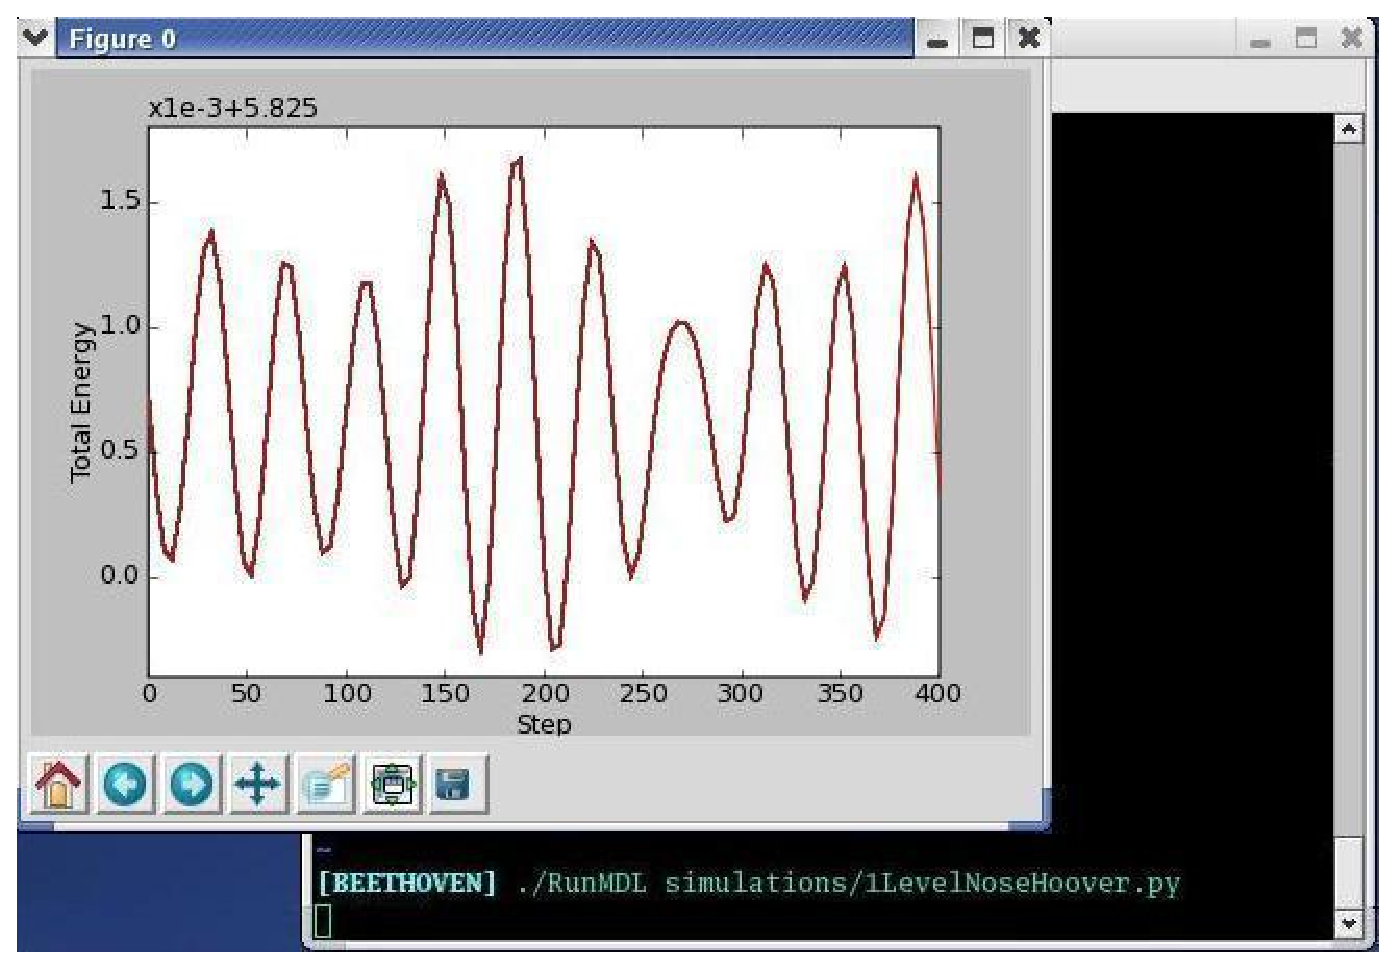
\includegraphics[width=12cm]{matplotlib2.eps}}
   \caption{Interactive plot of total energy while running an MDL simulation of united-atom butane. \label{fig:matplotlib}}
\end{figure}

\section{Propagation}

After setting up a physical system and a set of forces to evaluate,
the system can be propagate with time by applying a {\it propagator}
to the positions and velocities.  A propagator updates positions
and velocities using a {\it timestep} \begin{math}\Delta t\end{math}.
Each application of the propagator updates a system over biological
time \begin{math}\Delta t\end{math}, so {\it n} applications propagates
over time \begin{math} n \Delta t\end{math}.  \begin{math} \Delta t \end{math}
must of course be chosen carefully, a very low value results in longer
simulations but high values may result in instabilities or unacceptable
losses in accuracy by failing to account for fast frequency motions.
Certain propagators may make acceptable approximations and as a result 
allow for longer timesteps.

Your first step will be to construct an instance of the MDL
\texttt{Propagator} class, passing three objects as parameters:
a \texttt{Physical}, \texttt{Forces}, and \texttt{IO}:

\begin{verbatim}
prop = Propagator(phys, forces, io)
\end{verbatim}

Subsequently, the system can be propagated by invoking the 
\texttt{propagate} member function of class \texttt{Propagator}.
For single-timestepping (STS) propagation, the \texttt{propagate}
method accepts as parameters a uniquely identifying Python
string for the propagator name, an integer for the number of
steps to run, a floating point value for the timestep, and
a \texttt{ForceField} object for evaluation.  For example,
to propagate for 1 ps using a timestep of 0.5 fs using the
Leapfrog \cite{HoEa81} method (conserving number of atoms,
volume, and total energy):

\begin{verbatim}
prop.propagate(scheme="Leapfrog", steps=2000, dt=0.5, forcefield=ff)
\end{verbatim}

This will update the \texttt{Physical} and \texttt{Forces} objects
that were passed to the constructor of this \texttt{Propagator}.
\texttt{propagate} will also invoke any output routines specified
in the \texttt{IO} object passed to this constructor. There is one more
optional parameter for the \texttt{propagate} method, a Python dictionary
\texttt{params}.  Some propagators can accept extra parameters, and
some do not.  The Leapfrog method for example does not need any
other parameters, but Langevin dynamics (conserving number of
atoms, volume, and temperature) requires a damping coefficient
\begin{math}\gamma\end{math} for its frictional and random collision terms, 
and also a Kelvin temperature for the collision term.  MDL provides
an integrator \texttt{LangevinImpulse} \cite{SkIz02} for this purpose:

\begin{verbatim}
prop.propagate(scheme="LangevinImpulse", 
               steps=2000, 
               dt=0.5, 
               forcefield=ff,
               params={'gamma':3.0,
                       'temp':300})
\end{verbatim}


In either case defaults are always provided, so
you can always invoke a propagation scheme without providing extra
parameters and use default values.  MDL provides the following STS
propagation schemes, with corresponding parameters, data types
and default values:

\begin{enumerate}
\item {\bf Leapfrog}: The Leapfrog (or Velocity Verlet) method \cite{HoEa81}.  {\it Parameters: NONE}
\item {\bf PLeapfrog}: The Position Verlet method \cite{}.  {\it Parameters: NONE}
\item {\bf LeapfrogTruncatedShadow}: The Leapfrog method, which uses the solution of a nearby {\it Shadow Hamiltonian} \cite{ENSD05}.  {\it Parameters: NONE}
\item {\bf LangevinImpulse}: The Langevin Impulse method \cite{SkIz02}.  {\it Parameters: {\bf temp} (Kelvin temperature, floating point, 300), {\bf gamma} (damping coefficient, floating point, 91), {\bf seed} (random number seed, integer, 1234)}.
\item {\bf DMDLeapfrog}: Extension of the Leapfrog method to Langevin dynamics \cite{}.  {\it Parameters: Same as LangevinImpuse, plus {\bf iter} (number of velocity updates before calculating the dissipative term, integer, 5)}.
\item {\bf NoseNVTLeapfrog}: The Nose Hoover method \cite{Nose84, Hoov85}. {\it Parameters: {\bf temp} (Kelvin temperature, floating point, 300), {\bf inertia} (thermal inertia, floating point, 0.5), {\bf bathpos} (heat bath center of mass location, floating point, 1.0)}.  
\item {\bf CGMinimizer}: Non-linear conjugate gradient minimizer \cite{}.{\it Parameters: {\bf alpha} (Point where decrease is significant, floating point, 0.001), {\bf beta} (Point where directional derivative decrease is significant, floating point, 0.05), {\bf restart} (restart interval, integer, 0)}.  
\item {\bf NumericalDifferentiation}: Used to check force implementations by making a second approximation to forces by perturbing positions by some small value, recomputing potential energy and then using a Taylor series to estimate the force value.  Outputs the force error and Hessian.  {\it Parameters: {\bf epsilon} (Amount of perturbation, floating point, 1.0)}
\end{enumerate}


Each of the above STS integrators evaluates one set of forces per
step.  In some cases it may be desirable to evaluate two different
sets of forces at different frequencies, for example if one set
is more slowly varying than the other.  This can be done by
using a chain of one or more {\it multiple timestepping} (MTS)
propagators, sequentially evaluating faster varying forces at 
larger frequencies and the fastest using an STS propagator, terminating
the chain.

\subsection{Normal Mode Analysis}

MDL contains several built-in propagators to perform {\it normal
mode analysis}.  The frequencies of the normal modes of a system
are determined by the eigenvalues of the mass-reweighted Hessian
matrix (contains second derivatives of the potential).  The idea
of normal mode analysis is to divide a system into slow and fast
frequency modes, propagating the former with a propagator such
as Langevin Impulse and the latter using a more efficient Brownian
dynamics, relaxing their values around local energy minima.
The Normal Mode Langevin \cite{SPPI08} method does this using a 
three-level MTS propagation: with the outermost MTS propagator 
rediagonalizing the mass-reweighted Hessian, an inner MTS propagator
running Langevin dynamics on the slow modes, and the innermost
STS propagator performing energy minimization using mass-reweighted
steepest descent.  In this case you will need three \texttt{ForceField}
objects, assume they are bound to variable names \texttt{ff}, \texttt{ff2}
and \texttt{ff3}.  For MTS propagation, the member function \texttt{propagate}
of class \texttt{Propagator} accepts a \texttt{cyclelength} parameter, which will just
be an integer for a two-level scheme, or a Python list for three or more levels:

\begin{verbatim}
prop.propagate(scheme=['NormalModeDiagonalize', 
                       'NormalModeLangevin', 
                       'NormalModeMinimizer'],
               steps=20,
               cyclelength=[1,1],
               dt=4.0,
               forcefield=[ff, ff2, ff3],
               params={'NormalModeDiagonalize':{'reDiagFrequency':100,
                                                'minSteps':20,
                                                'minLim':0.1,
                                                'removeRand':1},
                       'NormalModeLangevin':{'firstmode':1,
                                             'numbermodes':22,
                                             'gamma':80,
                                             'seed':1234,
                                             'temperature':300},
                       'NormalModeMinimizer':{'minimlim':0.5,
                                              'simplemin':1}})
\end{verbatim}

Normal mode propagators accept a decent number of parameters, although
in many cases the defaults will be acceptable.  The outermost \texttt{NormalModeDiagonalize}
accepts a frequency to rediagonalize the mass-reweighted Hessian, the number of
minimization steps, a threshold at which to stop minimization, and a boolean value
which specifies whether or not the last random perturbation should be removed from
the system (this would come from the innermost propagator).  \texttt{NormalModeLangevin}
accepts parameters similar to \texttt{LangevinImpulse} (the Kelvin temperature,
damping coefficient and random seed), and in addition accepts a few more for the
number of fast frequency modes starting from a particular first mode (which will usually
be 1).  For the \texttt{NormalModeMinimizer}, once again a threshold is specified for
the potential energy deviation and a boolean value designating whether a simple
minimization is desired (1, default) or an exact minima projection.  Alternatively,
a Mori-Zwanzig \cite{} formalism can be used to project dynamics, which also
can output mode data into a directory:


\begin{verbatim}
prop.propagate(scheme=['NormalModeMori', 
                       'NormalModeRelax', 
                       'NormalModeBrownian'],
               steps=20,
               cyclelength=[1,1],
               dt=4.0,
               forcefield=[ff, ff2, ff3],
               params={'NormalModeMori':{'firstmode':1,
                                         'numbermodes':10,
                                         'gamma':80,
                                         'seed':1234,
                                         'temperature':300,
                                         'modeOutput':'modes'},
                       'NormalModeRelax':{'minimlim':0.5,
                                          'rediag':0,
                                          'simplemin':1},
                       'NormalModeBrownian':{'firstmode':11,
                                             'numbermodes':56,
                                             'gamma':420,
                                             'seed':1234,
                                             'temperature':300}})
\end{verbatim}

\newpage
\section{Examples}

Here we provide two examples of complete MDL simulation protocol scripts.  In addition, several more are available in the \texttt{simulations/} directory in the MDL framework.

\subsection{United Atom Butane in Vacuum for 1 ps, Leapfrog}

\begin{verbatim}

# A DRAFT OF A SIMULATION OF 4-ATOM BUTANE
# USING THE NEW STRUCTURE
from Physical import *
from Forces import *
from Propagator import *
from IO import *
from ForceField import *

# PHYSICAL SYSTEM
phys = Physical()
io = IO()
io.readPDBPos(phys, "data/UA_butane/UA_butane.pdb")
io.readPSF(phys, "data/UA_butane/UA_butane.psf")
io.readPAR(phys, "data/UA_butane/UA_butane.par")
phys.bc = "Periodic"
phys.cellsize = 6.5
phys.temperature = 300

# FORCES
forces = Forces()
ff = forces.makeForceField(phys, "charmm")


# OUTPUT
# PLOT KINETIC ENERGY EVERY 4 STEPS
# GENERATE SCREEN OUTPUT EVERY 2 STEPS
io.plots = {'kineticenergy':4}
io.screen = 2


# PROPAGATION
prop = Propagator(phys, forces, io)
prop.propagate(scheme="Leapfrog", steps=200, dt=0.5, forcefield=ff)
\end{verbatim}


\newpage
\subsection{Solvated Bovine Pancreatic Tripsin Inhibitor (BPTI) running Langevin Impulse using cutoffs}

\begin{verbatim}
# A DRAFT OF A SIMULATION OF 4-ATOM BUTANE
# USING THE NEW STRUCTURE
from Physical import *
from Forces import *
from Propagator import *
from IO import *
from ForceField import *



# PHYSICAL
phys = Physical()
io = IO()
io.readPDBPos(phys, "data/bpti_water_1101/bpti.pdb")
io.readPSF(phys, "data/bpti_water_1101/bpti.psf")
io.readPAR(phys, "data/bpti_water_1101/bpti.par")
phys.bc = "Periodic"
phys.cellsize = 5
phys.exclude = "scaled1-4"
phys.temperature = 0
phys.seed = 7536031

# FORCES
forces = Forces()
ff = forces.makeForceField(phys, "charmm")
ff.params['LennardJonesCoulomb'] = {'algorithm':'Cutoff',
                                    'switching':['C2', 'C1'],
                                    'cutoff':8.0}

# OUTPUT
# WRITE FILE bpti.energies EVERY 4 STEPS
# GENERATE SCREEN OUTPUT EVERY 2 STEPS
io.files = {'energies':('bpti.energies',4)}
io.screen = 2

# EXECUTE
prop = Propagator(phys, forces, io)
gamma = prop.propagate(scheme="LangevinImpulse", steps=2000, dt=0.1, 
                       forcefield=ff,
                       params={'LangevinImpulse':{'gamma':0.5}})



\end{verbatim}

Up to this point, all simulation protocols have used predefined propagation schemes.
Each of these propagation schemes was referenced using a uniqely identifying Python
string, and is implemented as precompiled machine code
for maximum efficiency.  However, the central purpose of MDL is to test {\it new}
numerical methods, and we now discuss (1) how to construct new propagators and
force calculators using pure Python and (2) how to equate a uniquely identifying
string with the new numerical method and couple this as a key within the internal
MDL propagator and force factories.


\chapter{Constructing New Propagators}

MDL provides a great deal of freedom in terms of acceptable implementations
of new propagation schemes.  In particular, you can choose the programming
style with which you are most familiar; if you prefer procedural programming
you can construct a propagator as a Python function, and if you like 
object-oriented design you can also construct a propagator as a Python class.
Each are recognizable by the MDL propagator factories, as long as the new
propagator has a uniquely defined Python string which does not serve as the
key for any other propagator.

\section{Propagator Factories}

Internally, MDL propagator factories map Python strings (keys) to 
{\it initialization methods}; that is, a method for constructing the new propagator.
In the case of Python functions, this is just a Python function handle; in the
case of Python classes, this is the constructor of the class.
In the \texttt{src/propagators} directory of the MDL framework, there are two
subdirectories, \texttt{classes} and \texttt{functions}.  The propagator
factory automatically searches these directories for Python-prototyped
propagation schemes, and loads all available modules.  Thus if you are constructing
a new propagator in Python, you will want to include its module in either
\texttt{classes} or \texttt{functions}, depending on which implementation
method you choose.  There are several example Python-prototyped propagators
in these directories.  In the \texttt{classes} folder, there are implementations
of Leapfrog \cite{HoEa81}, Br{\"u}nger-Brooks-Karplus (BBK, \cite{BrBk82}), the Hybrid Monte Carlo (HMC, \cite{})
sampling method, Nose-Poincar\'e \cite{}, and Recursive Multiple Thermostatting \cite{Swee04}, and
the MTS propagator Verlet-I/r-RESPA \cite{GRUB89A, GHWS91, TuBM92} (also known as {\it Impulse}).
For \texttt{functions}, we have included BBK, Leapfrog, Impulse, a simplified
version of Takahashi-Imada \cite{TaIm84}, and a velocity scaler which runs Velocity Verlet,
but includes one final scaling of velocities to keep the average kinetic energy
over all atoms constant.  These provide a wide range of examples which you can
use as a guide when constructing your own propagators.  Most importantly however, there
are two Python variables which you must define someplace in your new module: \texttt{name}
and \texttt{parameters}, in order for the factory to recognize your propagator.
Set \texttt{name} equal to the uniquely identifying Python string, and set \texttt{parameters}
equal to a Python tuple which alternates Python strings for the name of the variable,
and default values (see one of the examples for help).  For propagators implemented as Python classes, 
these variable names will become bound as member variables of the class.  For Python
functions, you will still need to pass them as formal parameters.  For instance, if you look
at \texttt{BBK.py}, which runs Langevin dynamics and thus needs the same parameters
as Langevin Impulse (a temperature, frictional coefficient and random number seed):

\begin{verbatim}
name="BBK"  
parameters=("temp", 300,
            "gamma", 2,
            "seed", 1234) 
\end{verbatim}

parameter names and defaults alternate in the Python tuple.  Note also that in
the implementation of class \texttt{BBK}, each of these variable names are used
at some point in the calculation, as data members of class \texttt{BBK} (thus
bound as attributes of \texttt{self}.


\section{Classes}

Constructing a propagator class first requires inheriting from either \texttt{STS}
(for single-timestepping propagators) or \texttt{MTS} for (multiple-timestepping).
As an example, the Python implementation of Leapfrog inherits from \texttt{STS}:

\begin{verbatim}
class LeapfrogPy(STS):
\end{verbatim}

while Impulse inherits from \texttt{MTS}:

\begin{verbatim}
class Impulse(MTS):
\end{verbatim}

Once the class has been declared, you can define any of three member functions 
which are recognized internally by MDL.  Recall that upon invoking
\texttt{propagate}, a user supplies a number of steps to execute the propagator.
These member functions are called automatically at various stages of propagation:   \\

1. \texttt{init}: Invoked once at the beginning of propagation. \\
\indent 2. \texttt{run}: Invoked at every step of propagation. \\
\indent 3. \texttt{finish}: Invoked once at the end of propagation. \\

Each of these member functions returns nothing and accepts three parameters:
a \texttt{Physical} object, a \texttt{Forces} object and a \texttt{Propagator} object.
In their definitions, they can access any attributes of these formal parameter objects,
along with any member attributes that were defined as parameters for this propagator.
At some point, these functions will likely update the \texttt{positions} and 
\texttt{velocities} data members of the \texttt{Physical} object, but of course
they may need other attributes like the \texttt{force} vector to accomplish this.
Note that matrix-vector operations can be performed to facilitate this process.
For example in the case of Leapfrog (or Velocity Verlet), recall that two
half-timestep updates of velocities (half-kicks) sandwich a full timestep
update of positions (kicks).  We can implement this functionality within 
a run member function.  Note that the \texttt{calculateForces} member
function will update the atomic \texttt{force} vector:

\begin{verbatim}
   def run(self, phys, forces, prop):
      phys.velocities += forces.force*0.5*self.dt*phys.invmasses
      phys.positions += phys.velocities*self.dt
      prop.calculateForces(forces)
      phys.velocities += forces.force*0.5*self.dt*phys.invmasses
\end{verbatim}

\texttt{MTS} propagators will be implemented similar except that you will
want to invoke some of the following member functions of \texttt{Propagator}:
\texttt{initNext}, \texttt{runNext}, and \texttt{finishNext}.
This is because MDL only actually invokes the outermost integrator on a call
to \texttt{propagate}.  The inner integrators are invoked at the proper
times in your implementation through calls to one of these functions.
For example, in the Python implementation of Impulse, we run the
inner integrator (faster frequency forces) and then calculate our own
slower frequency forces.  Note that \texttt{cyclelength} is automatically
bound as a member variable for \texttt{MTS} propagators:

\begin{verbatim}
prop.runNext(phys, forces, self.cyclelength)
prop.calculateForces(forces)
\end{verbatim}

\subsection{Modifiers}

Functionality of propagator objects can be slightly modified for
special cases using {\it modifiers}, which are Python functions
designed to be invoked at specific points in the propagation.
For example, we could modify a Leapfrog propagator to sample the NVT
ensemble by doing {\it velocity scaling}, which multiplies the 
velocities by \begin{math}\sqrt{T_0/T}\end{math} where 
\begin{math}T_0\end{math} is our target temperature, keeping
the average kinetic energy 
\begin{math} <KE> = \frac{3}{2}kT \end{math} constant.  We can define
a modifier for this:

\begin{verbatim}
def scaleVelocities(phys, forces, prop, obj):
   phys.velocities *= numpy.sqrt(obj.T0 / phys.temperature())
\end{verbatim}

The location at which a modifier is invoked depends on its 
{\it type}, which is specified at the point it is coupled to
a propagator.  The type of a modifier can be: \texttt{PreInit}, 
\texttt{PostInit}, \texttt{PreRun}, \texttt{PostRun}, 
\texttt{PreForce} or \texttt{PostForce}.  In this case we
would scale velocities at the end of propagation to prevent
further updates after the scaling and ensure proper Kelvin temperature,
so we would classify this as a \texttt{PostRun} modifier.
We then could construct a \texttt{VelocityScale} class which
inherits from \texttt{Leapfrog} but uses this modifier, by
defining a variable \texttt{modifiers} in the \texttt{VelocityScale}
module and assigning it a Python array of two-element tuples
which contain modifier names and types.  \texttt{T0} in this
case is our target temperature, and this becomes bound as
an attribute of class \texttt{VelocityScale}:


\begin{verbatim}
class VelocityScale(Leapfrog):
   pass

name="VelocityScale",
parameters=('T0', 300)
modifiers = [("scaleVelocities", "PostRun")]
\end{verbatim}


\section{Functions}

If procedural programming is more favorable for you than object-oriented,
you may prefer to implement a new propagator as a Python function instead
of a Python class.  In the case of a Python function, functionality
is not divided into initialization, execution and finishing routines like
classes, since everything is implemented as one function which is called
within \texttt{propagate}.  Propagator functions require a minimum of 
six formal parameters in the following order: a \texttt{Physical} object,
a \texttt{Forces} object, an \texttt{IO} object (note that you will
now need to manually invoke the member function \texttt{run} of \texttt{IO}
whenever you want output produced), number of steps, timestep (or cyclelength
for MTS, and \texttt{ForceField} object.  Following these are any extra parameter
names that you specified in the variable \texttt{parameters}, to be
recognized by the propagator factory.  Finally, if this propagator
is MTS, you must include a parameter for the next propagator in the 
chain (a Python function handle) and a formal parameter \texttt{*args}
for its parameters.  Thus for a BBK implementation, the header might
look something like this, if we had defined propagator parameters
\texttt{temp} (temperature), \texttt{gamma} and \texttt{seed}:

\begin{verbatim}
def bbk(phys, forces, prop, steps, dt, ff, temp, gamma, seed):
\end{verbatim}

Or for Impulse since it is an MTS propagator, we must add formal parameters
for the next propagator in the chain:

\begin{verbatim}
def impulse(phys, forces, io, steps, cyclelength, ff, nextprop, *args):
\end{verbatim}


We then can update system structures as with classes.  The only real
differences are that calculating forces is now done through the
\texttt{ForceField} object:

\begin{verbatim}
ff.calculateForces(phys, forces)
\end{verbatim}

And for MTS, the next propagator in the chain can simply be invoked
at the appropriate time.  Note that the same \texttt{Physical}, 
\texttt{Forces} and \texttt{IO} objects must be passed.  Propagator
functions cannot use modifiers.

\begin{verbatim}
nextinteg(phys, forces, io, *args)
\end{verbatim}


\chapter{Constructing New Forces}

Unlike propagators, new force calculators must be constructed as Python
classes.  We plan to add force functions eventually.  Any Python-prototyped
forces should be contained in the \texttt{src/forces} directory.  MDL
provides an example implementation of a {\it harmonic dihedral} force
as a Python class, which we now discuss.  This force effectively implements
a biasing potential which can allow sampling of traditionally unfavorable
areas of conformational space by restraining a system around a particular
angle value of one specific dihedral.  Of course multiple dihedrals
may be restrained by including this force more than once with different
target values.  A Python force class is declared in the usual way:

\begin{verbatim}
class HDForce:
\end{verbatim}

Python-prototyped forces must define two member functions: a constructor
and an \texttt{eval} method which takes no arguments and returns
nothing.  The harmonic dihedral restraint can be represented by
the following potential energy term:

\begin{equation}
V(\vec x) = k (\phi_{i}(\vec x) - \phi_{0}) ^ {2},
\label{eqn:harmd}
\end{equation}

where {\it i} is the dihedral number which we are restraining and 
\begin{math} \phi_{i}(\vec x) \end{math} is its dihedral angle value,
\begin{math} \phi_{0} \end{math} is the equilibrium or 'target'
dihedral angle value and {\it k} is a scaling factor.  To use this
restraint, you would need to know the values of {\it k}, {\it i}, and
\begin{math} \phi_{0} \end{math}.  Thus when defining the constructor
we would want the user to supply values for each of these variables
by passing them as formal parameters to the constructor, and binding their
names as data members of the new class \texttt{HDForce}.  In addition
we would want to pass any system structures which are necessary for
computing this force, i.e. the MDL \texttt{Physical} (for computing
the result) and \texttt{Forces} object (to populate the atomic force
vector):

\begin{verbatim}
def __init__(self, phys, forces, phi0, index, k):
    self.phys = phys
    self.forces = forces
    self.phi0 = phi0
    self.index = index
    self.k = k
\end{verbatim}

The job of the \texttt{eval} method is to compute both
energies and forces and populate the \texttt{energies} data 
member of \texttt{Forces} and the atomic force vector \texttt{force}.
The \texttt{eval} method does not accept any extra parameters,
other than the \texttt{self} pointer which all member functions
must accept.  Thus all computation must be performed by data
members of self (and thus all data member bindings should be performed
in the constructor):

\begin{verbatim}
  def eval(self):
\end{verbatim}

In the above case, we first compute the potential energy term
according to Eq. (\ref{eqn:harmd}).  We first compute the difference
between the current value of dihedral {\it i} and its target value
\begin{math} \phi_{0} \end{math} and accumulate the resulting 
potential energy value into the dihedral energy term of the
\texttt{energies} data member of \texttt{Forces}:

\begin{verbatim}
    diff = self.phys.angle(self.index) - self.phi0;
    self.forces.energies.addDihedralEnergy(self.k * diff * diff)
\end{verbatim}

Next, the force on each atom must be computed as:

\begin{equation}
F_{i} = \frac{\partial U}{\partial \phi} \frac{\partial \phi}{\partial x_{i}}.
\end{equation}

Since there are only four atoms involved in the dihedral
being restrained, the atomic force vector will only be modified in four 
locations.  Computing \begin{math}\frac{\partial U}{\partial \phi}\end{math}
is trivial:

\begin{verbatim}
    dVdPhi = 2 * self.k * diff
\end{verbatim} 

Computing \begin{math}\frac{\partial \phi}{\partial x_{i}}\end{math}
is a bit more complicated:

\begin{equation}
  \nabla \phi =  \frac{ 1 }{ \cos(\phi) } \nabla \left( \frac{ \vec{C}
\cdot \vec{B} }{ |\vec{C}| |\vec{B}| } \right),
\end{equation}

where:

\begin{eqnarray*}
  \vec{A} = \Vr{ij} \times \Vr{jk}   \\
  \vec{B} = \Vr{jk} \times \Vr{kl}   \\
  \vec{C} = \Vr{jk} \times \vec{A}.
\end{eqnarray*}

We thus must first compute the distance
vectors for applicable pairs of atoms in the dihedral, then
set the values of \begin{math}\vec{A}\end{math}, 
\begin{math}\vec{B}\end{math}.
We make use of the \texttt{cross} function provided by
numpy to compute the cross product of two three-element vectors:

\begin{verbatim}
    i = self.phys.angle(self.i-1).atom1 - 1
    j = self.phys.angle(self.i-1).atom2 - 1
    k = self.phys.angle(self.i-1).atom3 - 1
    l = self.phys.angle(self.i-1).atom4 - 1
    rij = self.phys.positions[j*3:j*3+3] - self.phys.positions[i*3:i*3+3]
    rkj = self.phys.positions[j*3:j*3+3] - self.phys.positions[k*3:k*3+3]
    rkl = self.phys.positions[l*3:l*3+3] - self.phys.positions[k*3:k*3+3]
    A = numpy.cross(rij, rkj)
    B = numpy.cross(rkj, rkl)
\end{verbatim}

Finally we compute the force on each atom \texttt{fi}, \texttt{fj}, etc.
and accumulate these into the atomic force vector, data member
\texttt{force} of \texttt{Forces}:

\begin{verbatim}
    fi = A * (-dVdPhi * norm(rkj) / norm2(A));
    fl = B * (dVdPhi * norm(rkj) / norm2(B));
    fj =   fi * (-1 + numpy.dot(rij, rkj)/norm2(rkj)) 
         - fl * (numpy.dot(rkl, rkj)/norm2(rkj));
    fk = - (fi + fj + fl);

    self.forces.force[atomI*3:atomI*3+3] += fi
    self.forces.force[atomJ*3:atomJ*3+3] += fj
    self.forces.force[atomK*3:atomK*3+3] += fk
    self.forces.force[atomL*3:atomL*3+3] += fl
\end{verbatim}

Since Python-prototyped forces are not by default recognized as CHARMM
forces, instances of their classes must be explicitly constructed in
the simulation protocol, passing all necessary parameters to the 
constructor, i.e.:

\begin{verbatim}
hd = HDForce(phys, forces, 3.1, 11, 5.0)
\end{verbatim} 

To add the object to a \texttt{ForceField} for evaluation, you can pass an 
instance as a formal parameter to the \texttt{ForceField}
member function \texttt{addPythonForce}:

\begin{verbatim}
ff.addPythonForce(hd)
\end{verbatim}


\chapter{MDL Licensing}

MDL is distributed as a tier of the ProtoMol framework, and all licensing,
conditions and regulations of ProtoMol apply to MDL as well.  


\section{Contact Information}

The best contact path for licensing issues is by e-mail to  
{\it protomol@cse.nd.edu} or send correspondence to: \\ \\
\ProtoMol Team\\
c/o Prof. Jes\'{u}s A. Izaguirre\\
Laboratory for Computational Life Sciences\\
Department of Computer Science and Engineering\\
University of Notre Dame\\
384 Fitzpatrick Hall of Engineering\\
Notre Dame, Indiana 46556 USA


\bibliographystyle{plain}
\bibliography{lcls}                                     
%%%%%%%%%%%%%%%%%%%%%%%%%%%%%%%%%%%%%%%%%%%%%%%%%%%%%%%%%%%%%%%%%%%%%%%%%



\end{document}
